\documentclass{standalone}

\usepackage{tikz}
\usetikzlibrary{arrows}

\usepackage{ifthen}

\begin{document}
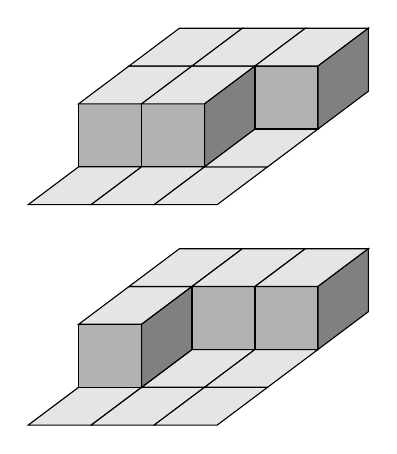
\begin{tikzpicture}[scale=(0.8)]
\def\a{.8}
\def\b{.6}

\newcommand{\tikzsquare}[4]{
	\ifthenelse{#4=1} {
	\filldraw[fill=black!50!, draw=black]  (#1+\a*#3,#2+\b*#3) -- (#1+\a*#3+\a,#2+\b*#3+\b) -- (#1+\a*#3+\a,#2+\b*#3+1+\b) -- (#1+\a*#3,#2+\b*#3+1) -- cycle;
	} {}
	\ifthenelse{#4=2} {
	\filldraw[fill=black!10!, draw=black] (#1+\a*#3,#2+\b*#3) -- (#1+\a*#3+\a,#2+\b*#3+\b) -- (#1+\a*#3+1+\a,#2+\b*#3+\b) -- (#1+\a*#3+1,#2+\b*#3) -- cycle;
	} {}
	\ifthenelse{#4=3} {
	\filldraw[fill=black!30!, draw=black](#1+\a*#3,#2+\b*#3) -- (#1+\a*#3,#2+\b*#3+1) -- (#1+\a*#3+1,#2+\b*#3+1) -- (#1+\a*#3+1,#2+\b*#3) -- cycle;
	} {}
}

\tikzsquare{0}{0}{0}{2};
\tikzsquare{0}{0}{1}{3};
\tikzsquare{0}{1}{1}{2};
\tikzsquare{0}{1}{2}{2};

\tikzsquare{1}{0}{0}{2};
\tikzsquare{1}{0}{1}{2};
\tikzsquare{1}{0}{1}{1};
\tikzsquare{1}{0}{2}{3};
\tikzsquare{1}{1}{2}{2};

\tikzsquare{2}{0}{0}{2};
\tikzsquare{2}{0}{1}{2};
\tikzsquare{2}{0}{2}{3};
\tikzsquare{2}{1}{2}{2};
\tikzsquare{3}{0}{2}{1};

\begin{scope}[yshift=3.5cm] %[xshift=6cm] %

\tikzsquare{0}{0}{0}{2};
\tikzsquare{0}{0}{1}{3};
\tikzsquare{0}{1}{1}{2};
\tikzsquare{0}{1}{2}{2};

\tikzsquare{1}{0}{0}{2};
\tikzsquare{1}{0}{1}{3};
\tikzsquare{1}{1}{1}{2};
\tikzsquare{1}{1}{2}{2};

\tikzsquare{2}{0}{0}{2};
\tikzsquare{2}{0}{1}{1};
\tikzsquare{2}{0}{1}{2};
\tikzsquare{2}{0}{2}{3};
\tikzsquare{2}{1}{2}{2};
\tikzsquare{3}{0}{2}{1};

\end{scope}
\end{tikzpicture}
\end{document}